
\chapter*{Introduction}


\lgf{L'internet des Objets ne va pas seulement ajouter une nouvelle catégorie d'équipements au réseau, il va également modifier la mise en \oe{}uvre des protocoles.  Il faut donc être à la fois différent mais identique, disruptif mais conservateur. 
L'Internet des Objets constitue une évolution majeure des protocoles mondiaux pour répondre à deux défis fondamentaux : être économe en énergie et surtout être interopérable ; c'est-à-dire permettre aux Objets de s’intégrer facilement dans les systèmes d’information existants et au final l'information produite banalisée. }
\lge{The Internet of Things will not only add a new category of equipment to the network, it will also change the way protocols are implemented.  So we need to be different but the same, disruptive but conservative. 
The Internet of Things is a major evolution of global protocols to meet two fundamental challenges: to be energy efficient and above all to be interoperable; that is to say, to enable Objects to be easily integrated into existing information systems and ultimately to make the information produced widely available.}

\lgf{L'IoT modifie également la manière d'enseigner. Jusqu'à présent cet enseignement était très stratifié, on montrait en cours magistral comment fonctionne les protocoles, comment ils s'organisent. La mise en \oe{}uvre pratique portait plutôt sur la configuration des équipements d'interconnexion comme les routeurs. La vision traditionnelle consiste a bien séparer les fonctionnalités. Les protocoles sont empilés les uns sur les autres avec les fonctionnalités comme le codage de l'information, sur lesquelles reposent l'aiguillage de l'information et au sommet les  applications. Chaque protocole dans cet empilement  indépendant les uns des autres et des frontières très strictes.} 
\lge{The IoT also changes the way we teach. Until now, this teaching was very stratified, with lectures showing how the protocols work and how they are organized. The practical implementation was more concerned with the configuration of interconnection equipment such as routers. The traditional vision consists in separating the functionalities. The protocols are stacked one on top of the other with the functionalities such as the coding of information, on which the routing of information is based, and at the top the applications. Each protocol in this stack is independent of the others and has very strict boundaries.}

~

\lgf{Cette vision est à revoir pour l'Internet des objets, les faibles capacités en mémoire, la nature des liens de communication font qu'il est difficile de se spécialiser dans un seul domaine. Ainsi, j'espérais avoir oublié pour toujours les aspects traitement du signal ou électronique en quittant l'université. Or pour concevoir un objet une approche pluridisciplinaire est essentielle, il faut donc à la fois appréhender des concepts électroniques aussi bien en terme de place que de consommation électrique, de traitement du signal car les signaux sont généralement très faibles, sans oublier les problèmes traditionnels en réseaux comme le routage, l'auto-configuration ou la sécurité. Il faut également avoir un \oe{}il sur les  applicatifs~:  comment les données sont représentées et codées lors de leur transmission et comment elles peuvent interagir avec des services existants. }
\lge{This vision has to be revised for the Internet of Things, the low memory capacities, the nature of the communication links make it difficult to specialize in only one field. Thus, I hoped to have forgotten forever the signal processing or electronic aspects when I left the university. However, in order to design an object, a multidisciplinary approach is essential, so you have to understand electronic concepts in terms of space as well as power consumption, signal processing because the signals are generally very weak, without forgetting traditional network problems such as routing, auto-configuration or security. It is also necessary to have an eye on the applications: how the data are represented and coded during their transmission and how they can interact with existing services. }

\lgf{L'Objet en lui même n'est qu'une petite partie du problème, il va envoyer un flux d'information plus ou moins important vers des serveurs qui seront chargés de les analyser, de les stocker, de trouver des tendances. Les petits ruisseaux faisant les grandes rivières, il faut que ces serveurs ou les réseaux qui y conduisent soient correctement dimensionnés. Mais également que le coût pour la gestion d'un objet soit très faible sinon en les cumulant sur des millions d'objets il peuvent être un frein au déploiement.}
\lge{The Thing itself is only a small part of the problem, it will send a more or less important flow of information to servers that will be responsible for analyzing, storing and finding trends. Since small streams make big rivers, these servers or the networks that lead to them must be correctly sized. But also that the cost of managing an object is very low, otherwise the cumulative cost of millions of objects can be a barrier to deployment..}


~

\lgf{Ce livre est le fruit des expériences que nous avons eu avec les ateliers de fabrication, et d'une constatation que le réseau est souvent le parent pauvre à la fois des applications créées mais également du support que l'on trouve sur ces plates-formes; les communications sont vues dans une optique de l'application, sans prendre en compte une vision d'interopérabilité plus globale conduisant au concept d'Internet des Objets. Ceci peut se comprendre car les piles protocolaires de l'Internet sont relativement importantes et dans un environnement restreint, il est plus facile de s'en débarrasser. Néanmoins, ces piles protocolaires ont un avantage, elles favorisent la communication entre les constituants du réseau. Ainsi, il est possible de piloter un objet a partir de son ordinateur portable, les données peuvent être envoyées sur des serveurs pour être traitées,... }
\lge{This book is the result of the experiences we had with the FabLabs, and of an observation that the network is often the poor relation both of the applications created and of the support found on these platforms; communications are seen from an application perspective, without taking into account a more global vision of interoperability leading to the concept of the Internet of Things. This is understandable because the protocol stacks of the Internet are relatively large and in a restricted environment, it is easier to get rid of them. Nevertheless, these protocol stacks have an advantage, they promote communication between the network components. Thus, it is possible to control an object from its laptop, data can be sent to servers to be processed,... }

\lgf{La richesse des possibilités de communication va permettre de créer des services innovants. Il faut aussi que les piles protocolaires s'adaptent. C'est ce que font de nombreux organismes dont l'IETF qui standardise les protocoles utilisés dans l'Internet.}
\lge{The variety of communication possibilities will allow the creation of innovative services. The protocol stacks must also adapt. This is what many organizations are doing, including the IETF, which standardizes the protocols used in the Internet.}
~
~



\lgf{Cet ouvrage est une adaptation du MOOC Programmer L'Internet des Objets sur Coursera. Il va couvrir les technologies, architectures et protocoles nécessaires pour la réalisation de bout en bout de la collecte d’informations sur des réseaux dédiés à l’IoT à la structuration de la donnée et à son traitement.}
\lge{This book is an adaptation of the MOOC Programming the Internet of Things on Coursera. It will cover the technologies, architectures and protocols needed for the end-to-end realization of information collection on networks dedicated to the IoT to the structuring of the data and its processing.}

\lgf{Vous allez notamment~:}
\lge{You're going to include:}
\begin{itemize}
\item 
    \lgf{découvrir une nouvelle catégorie de réseaux appelée LPWAN dont Sigfox et LoRaWAN sont les représentant les plus connus~;}
    \lge{discover a new category of networks called LPWAN of which Sigfox and LoRaWAN are the best known representatives~;}
\item 
    \lgf{voir l’évolution de la pile protocolaire de l’internet qui passe de IPv4/TCP/HTTP à IPv6/UDP/ CoAP tout en préservant le concept REST basé sur des ressources identifiées sans ambiguïté par des URI~;}
    \lge{see the evolution of the internet protocol stack from IPv4/TCP/HTTP to IPv6/UDP/CoAP while preserving the REST concept based on resources unambiguously identified by URI;}
\item 
    \lgf{expliquer comment CBOR peut être utilisé pour structurer des données complexes en complément de JSON~;}
    \lge{explain how CBOR can be used to structure complex data in addition to JSON;}
\item 
    \lgf{enfin JSON-LD et la base de données MongoDB nous permettront de manipuler aisément l’information collectée. Ainsi, nous introduirons les techniques essentielles pour valider statistiquement les données collectées.}
    \lge{Finally JSON-LD and the MongoDB database will allow us to easily manipulate the collected information. Thus, we will introduce the essential techniques to statistically validate the collected data.}

\end{itemize}
\lgf{À travers ce cours, vous apprendrez à programmer un Objet économe en énergie et interopérable avec d'autres Objets.}
\lge{Through this course, you will learn how to program an energy efficient Thing that is interoperable with other Things.}

\clearpage

\section *{\lgf{Materiel}\lge{Hardware}}

 \begin{wrapfigure}{r}{5.5cm}
\centerline{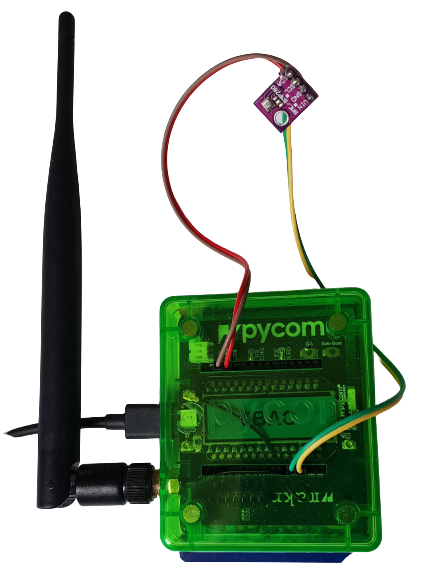
\includegraphics[width=.4\columnwidth]{Pictures/pycom-bme.png}}
\end{wrapfigure}

\lgf{Il n'est pas nécessaire d'avoir du matériel pour faire la plupart des exercices et expérimenter les concepts. A peu près tout peut se faire avec des scripts Python, mais ce n'est pas aussi amusant que les expérimentations en vrai. En particulier pour découvrir la magie des réseaux radios longue portée. C'est pour cela que nous allons utiliser le matériel suivant~:}
\lge{You don't need hardware to do most of the exercises and experiment with the concepts. Just about everything can be done with Python scripts, but it's not as much fun as experimenting in real life. Especially when it comes to discovering the magic of long range radio networks. That's why we will use the following material:}

\begin{itemize}
\item  
    \lgf{un  \fulluri{LoPy4}{https://pycom.io/product/lopy4/} -\textit{Pycom - Quadruple Bearer MicroPython enabled Dev Board} ; Attention : prendre l'option \textit{With headers}}
    \lge{a  \fulluri{LoPy4}{https://pycom.io/product/lopy4/} -\textit{Pycom - Quadruple Bearer MicroPython enabled Dev Board} ; Caution: take the option \textit{With headers}}

\item
    \lgf{une  \fulluri{Expansion Board 3.0}{https://pycom.io/product/expansion-board-3-0/} - Pycom - \textit{Compatible with Pycom Multi-Network IoT}~;}
    \lge{A  \fulluri{Expansion Board 3.0}{https://pycom.io/product/expansion-board-3-0/} - Pycom - \textit{Compatible with Pycom Multi-Network IoT};}

\item 
    \lgf{une \fulluri{antenne LoRa}{https://pycom.io/product/lora-868mhz-915mhz-sigfox-antenna-kit/} (868MHz/915MHz) \& Sigfox Antenna Kit - Pycom avec son petit fil permettant de la connecter au LoPy~;}
    \lge{une \fulluri{LoRa Antenna}{https://pycom.io/product/lora-868mhz-915mhz-sigfox-antenna-kit/} (868MHz/915MHz) \& Sigfox Antenna Kit - Pycom with its small wire allowing to connect it to LoPy;}


\item 
    \lgf{un \fulluri{boitier}{https://pycom.io/product/pycase-clear/}, mais ce n'est pas indispensable, si vous n'êtes pas soigneux \textit{Pycase Clear - Fits Pycom IoT Dev Boards, Expansion Board \& Antenna kit} ;}
    \lge{a \fulluri{box}{https://pycom.io/product/pycase-clear/},but it is not necessary, if you are not careful with your device \textit{Pycase Clear - Fits Pycom IoT Dev Boards, Expansion Board \& Antenna kit};}

\item 
    \lgf{un capteur \fulluri{BME280 3v3}{https://boutique.semageek.com/fr/704-capteur-de-pression-temperature-humidite-bme280-3009052078446.html}  Capteur de pression temperature humidite BME280 - Boutique Semageek ou \fulluri{BME280 3.3}{https://fr.aliexpress.com/item/1005002387867504.html?spm=a2g0o.productlist.0.0.580f7c3elwXr70&algo_pvid=bbd88dd7-92c5-4904-a4e7-6045b186dbd6&algo_expid=bbd88dd7-92c5-4904-a4e7-6045b186dbd6-1&btsid=0b0a182b16193744192742943e5955&ws_ab_test=searchweb0_0,searchweb201602_,searchweb201603_};}
    \lge{A sensor \fulluri{BME280 3v3}{https://boutique.semageek.com/fr/704-capteur-de-pression-temperature-humidite-bme280-3009052078446.html}  Capteur de pression temperature humidite BME280 - Boutique Semageek or \fulluri{BME280 3.3}{https://fr.aliexpress.com/item/1005002387867504.html?spm=a2g0o.productlist.0.0.580f7c3elwXr70&algo_pvid=bbd88dd7-92c5-4904-a4e7-6045b186dbd6&algo_expid=bbd88dd7-92c5-4904-a4e7-6045b186dbd6-1&btsid=0b0a182b16193744192742943e5955&ws_ab_test=searchweb0_0,searchweb201602_,searchweb201603_};}

\item 
    \lgf{un câble USB (USB 2.0A to micro B 2.0 1.5 m)~;}
    \lge{a USB cable (USB 2.0A to micro B 2.0 1.5 m);}

\item 
    \lgf{des câbles \fulluri{dupont mâle-femelle}{https://www.amazon.fr/cable-dupont/s?k=cable+dupont} }
    \lge{\fulluri{dupont male-femelle}{https://www.amazon.fr/cable-dupont/s?k=cable+dupont} cable}
\end{itemize}

  \vspace{1em}


\lgf{Le LoPy propose un an d'abonnement gratuit au réseau Sigfox, c'est suffisant pour expérimenter. Un abonnement annuel coûte une dizaine d'euros. Par contre, accéder à un réseau LoRaWAN est plus problématique. Les offres des opérateurs ne sont pas toujours adaptées et la couvertures des réseaux communautaires n'est pas complète. Mais vous pouvez étendre cette couverture en installant votre propre antenne LoRa pour moins d'une centaine d'euros. Nous utiliserons aussi la solution proposée par Pycom.}
\lge{LoPy offers a free one-year subscription to the Sigfox network, which is enough to experiment. An annual subscription costs about ten euros. On the other hand, accessing a LoRaWAN network is more problematic. The offers of the operators are not always adapted and the coverage of the community networks is not complete. But you can extend this coverage by installing your own LoRa antenna for less than a hundred euros. We will also use the solution proposed by Pycom.}

\lgf{Pour cela il faut~:}
\lge{To do this you need:}

\begin{itemize}
    \item 
        \lgf{une carte d'extension \fulluri{pygate}{https://pycom.io/product/pygate/}~;}
        \lge{an extension board \fulluri{pygate}{https://pycom.io/product/pygate/};}
    \item 
        \lgf{un LoPy comme précédement ou un un \fulluri{wi-py}{https://pycom.io/product/wipy-3-0/} un peu moins cher~;}
        \lge{a LoPy as before or a slightly cheaper \fulluri{wi-py}{https://pycom.io/product/wipy-3-0/};}
    \item 
        \lgf{un \fulluri{joli boitier}{https://pycom.io/product/pygate-case/} pour faire pro~;}
        \lge{a \fulluri{pretty box}{https://pycom.io/product/pygate-case/} to look professional;}
        
    \item 
        \lgf{son \fulluri{antenne avec son câble}{https://pycom.io/product/lora-868mhz-915mhz-sigfox-antenna-kit/}~;}
        \lge{its \fulluri{antenna with its cable}{https://pycom.io/product/lora-868mhz-915mhz-sigfox-antenna-kit/}~;}
    \item 
        \lgf{et cette fois-ci un câble USB-C.}
        \lge{and this time a USB-C cable.}
\end{itemize}

\lgf{\section{Ressources disponibles}}
\lge{\section{Available resources}}


\lgf{Ce livre en Open Source est accessible sur \url{https://github.com/ltn22/PLIDO_BOOK} en version française et anglaise. Les remarques et les commentaires peuvent être remontés en utilisation les outils de Github comme les \textit{Issue} et les \textit{Pull requests}. }
\lge{This Open Source book is available on \url{https://github.com/ltn22/PLIDO_BOOK} in French and English version. Remarks and comments can be sent back using Github tools like \textit{Issue} and \textit{Pull requests}. }

  \vspace{1em}


\lgf{Les vidéos référencées dans ce livre sont également disponibles sur Youtube \url{https://www.youtube.com/playlist?list=PLwy4KbYJoKLWeonJ8c5U6CLrxs_pZQi3q}. Et comme disent les Youtubers, n'oubliez pas de liker les videos et de vous abonner à la chaîne. }
\lge{The videos referenced in this book are also available on Youtube \url{https://www.youtube.com/playlist?list=PLwy4KbYJoKLWeonJ8c5U6CLrxs_pZQi3q}. And as the Youtubers say, don't forget to like the videos and subscribe to the channel. }

  \vspace{1em}


\lgf{Finalement, une version plus interactive, sous forme de MOOC est accessible ici \url{https://bit.ly/3Ku0aL8}. Le MOOC permet plus d'interactivités avec des forum pour directement poser des questions et des animations pour mieux configurer le système.  }
\lge{Finally, a more interactive version, in the form of a MOOC, is available here : \url{https://bit.ly/3Ku0aL8}. The MOOC allows more interactivity with forums to directly ask questions and animations to better configure the system.  }

\lgf{\section{Auteurs}}
\lge{\section{Authors}}


\begin{wrapfigure}{r}{6cm}
\centerline{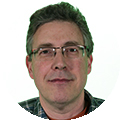
\includegraphics[width=.2\columnwidth]{Pictures/Laurent-Toutain.jpeg}}
\end{wrapfigure} 
\noindent
\lgf{Laurent Toutain est professeur au département Systèmes Réseaux, Cybersécurité et Droit du numérique d'IMT Atlantique, une école de l'institut Mines-Télécom.
Il est membre de l’équipe OCIF (Objets Communicants - Internet du Futur) qui se focalise sur les évolutions protocolaires et architecturales de l’internet liées à la conception de nouveaux services (Smart grid, vêtements intelligents…). Après avoir travaillé sur le protocole IPv6 et les mécanismes de transition dans différents environnements, il s’intéresse actuellement à leur intégration dans l'internet des objets. Il contribue également aux Fab Labs pour l’adoption de ces protocoles. Il est l'auteur de plusieurs livres de référence sur les réseaux.}
\lge{Laurent Toutain is a professor in the Network Systems, Cybersecurity and Digital Law department at IMT Atlantique, a school of the Mines-Telecom Institute.
He is a member of the OCIF team (Communicating Objects - Internet of the Future) which focuses on protocol and architectural evolutions of the Internet related to the design of new services (Smart grid, smart clothes...). After having worked on the IPv6 protocol and transition mechanisms in different environments, he is currently interested in their integration in the Internet of Things. He also contributes to Fab Labs for the adoption of these protocols. He is the author of several reference books on networks.}

  \vspace{3em}

 
\begin{wrapfigure}{r}{5cm}
\centerline{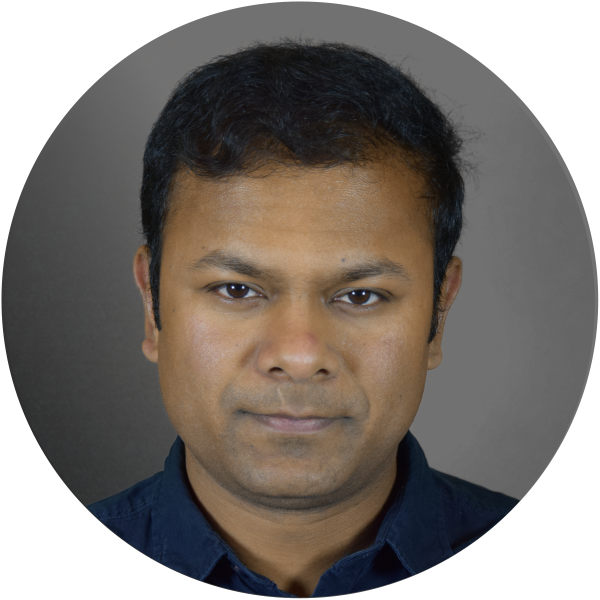
\includegraphics[width=.2\columnwidth]{Pictures/Kamal_Singh.png}}
\end{wrapfigure} 
Kamal Singh est Maitre de Conférences à Télécom Saint-Étienne où il dispense des cours de réseaux informatiques et de réseaux d’opérateurs. Il fait également partie de l’équipe de recherche Data Intelligence du Laboratoire Hubert Curien. Son travail porte sur l’internet des objets, les villes intelligentes, le Big Data, le Web sémantique, la qualité de l’expérience et le software defined networking.

  \vspace{7em}

\clearpage
\begin{wrapfigure}{r}{5cm}
\centerline{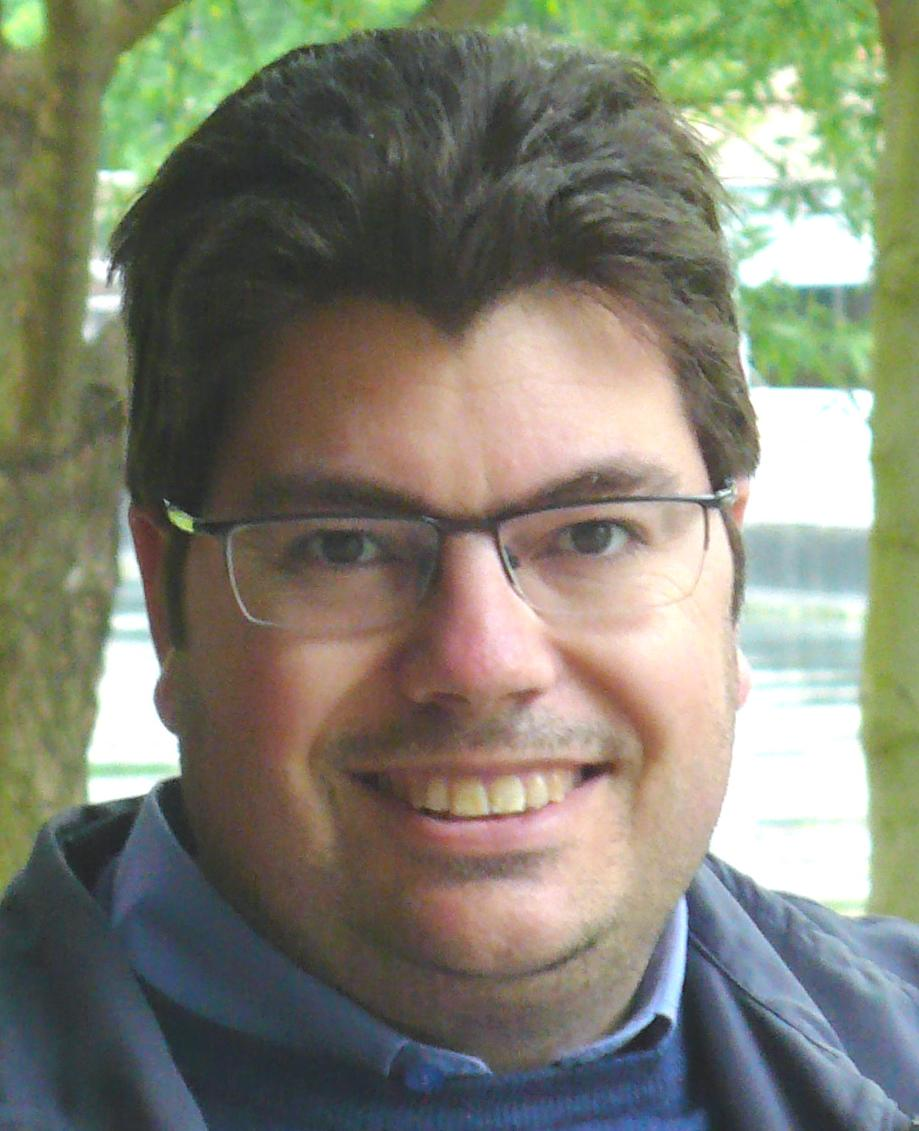
\includegraphics[width=.2\columnwidth]{Pictures/Photo_Marc_Girod_Genet.jpeg}}
\end{wrapfigure} 
\lgf{Marc Girod Genet est professeur associé à Télécom SudParis et chercheur associé CNRS-SAMOVAR (UMR 5157), au sein duquel il anime la thématique transverse sur l’énergie. Ses axes de recherche englobent notamment les réseaux personnels (réseaux de capteurs et architectures de mesures inclus), les communications M2M et les architectures de type IoT/WoT, les modèles de données sémantiques et les ontologies. Marc est par ailleurs impliqué dans des activités de standardisations au sein de l’AIOTI (Alliance for Internet of Things Innovation) et de l’ETSI (rapporteur, TC SmartBAN). Il a reçu en 2010 le prix spécial du jury « Croissance verte numérique » pour ses travaux sur les réseaux électriques intelligents et la gestion de la consommation d’énergie (un de ses deux domaines d’application avec la eSanté).}
\lge{Marc Girod Genet is an associate professor at Télécom SudParis and a CNRS-SAMOVAR associate researcher (UMR 5157), where he leads the transverse theme on energy. His research interests include personal networks (including sensor networks and measurement architectures), M2M communications and IoT/WoT architectures, semantic data models and ontologies. Marc is also involved in standardization activities within AIOTI (Alliance for Internet of Things Innovation) and ETSI (rapporteur, TC SmartBAN). In 2010, he received the special "Digital Green Growth" jury award for his work on smart grids and energy management (one of his two application areas along with eHealth).}

  \vspace{5em}


\begin{wrapfigure}{r}{5cm}
\centerline{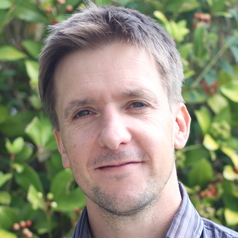
\includegraphics[width=.2\columnwidth]{Pictures/PatrickMaille.jpeg}}
\end{wrapfigure} 
\lgf{Patrick Maillé est professeur au département Systèmes Réseaux, Cybersécurité et Droit du numérique d'IMT Atlantique, une école de l'institut Mines-Télécom.
Diplômé de l’école polytechnique et Télécom ParisTech, il a soutenu sa thèse à Télécom Bretagne (maintenant IMT Atlantique) en 2005. Ses travaux de recherche portent sur l'économie des réseaux de télécommunication à l'aide d'outils de mathématiques appliquées et d'économie (notamment la théorie des jeux).}
\lge{Patrick Maillé is a professor in the Network Systems, Cybersecurity and Digital Law department of IMT Atlantique, a school of the Mines-Telecom Institute.
A graduate of the Ecole Polytechnique and Télécom ParisTech, he defended his thesis at Télécom Bretagne (now IMT Atlantique) in 2005. His research work focuses on the economics of telecommunication networks using applied mathematics and economics tools (notably game theory).}

  \vspace{5em}

\clearpage
\begin{wrapfigure}{r}{5cm}
\centerline{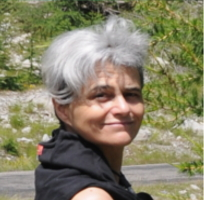
\includegraphics[width=.2\columnwidth]{Pictures/batton.jpeg}}
\end{wrapfigure} 

\lgf{Mireille Batton-Hubert est Professeure à l'École Nationale Supérieure des Mines de Saint Étienne, au centre d’enseignement et de recherche, l'institut Henri Fayol. Elle est responsable de l'équipe Génie Mathématique et Industriel (GMI) et rattachée à l'UMR Limos.
Le département Génie Mathématique et Industriel vise à proposer des méthodes quantitatives d’évaluation de la performance globale des entreprises et de leurs produits. Il rassemble des compétences allant des mathématiques appliquées au génie industriel.Le département Génie Mathématique et Industriel vise à proposer des méthodes quantitatives d’évaluation de la performance globale des entreprises et de leurs produits. Il rassemble des compétences allant des mathématiques appliquées au génie industriel.Le département Génie Mathématique et Industriel vise à proposer des méthodes quantitatives d’évaluation de la performance globale des entreprises et de leurs produits. Il rassemble des compétences allant des mathématiques appliquées au génie industriel.}
\lge{Mireille Batton-Hubert is a Professor at the École Nationale Supérieure des Mines de Saint Étienne, at the teaching and research center, the Henri Fayol Institute. She is in charge of the Mathematical and Industrial Engineering team (GMI) and is attached to the UMR Limos.
The Mathematical and Industrial Engineering department aims to propose quantitative methods for evaluating the overall performance of companies and their products. The Mathematical and Industrial Engineering department aims to propose quantitative methods for evaluating the overall performance of companies and their products. The Mathematical and Industrial Engineering department aims to propose quantitative methods for evaluating the overall performance of companies and their products. It brings together skills ranging from applied mathematics to industrial engineering.}

 
   \vspace{5em}

\begin{wrapfigure}{r}{5cm}
\centerline{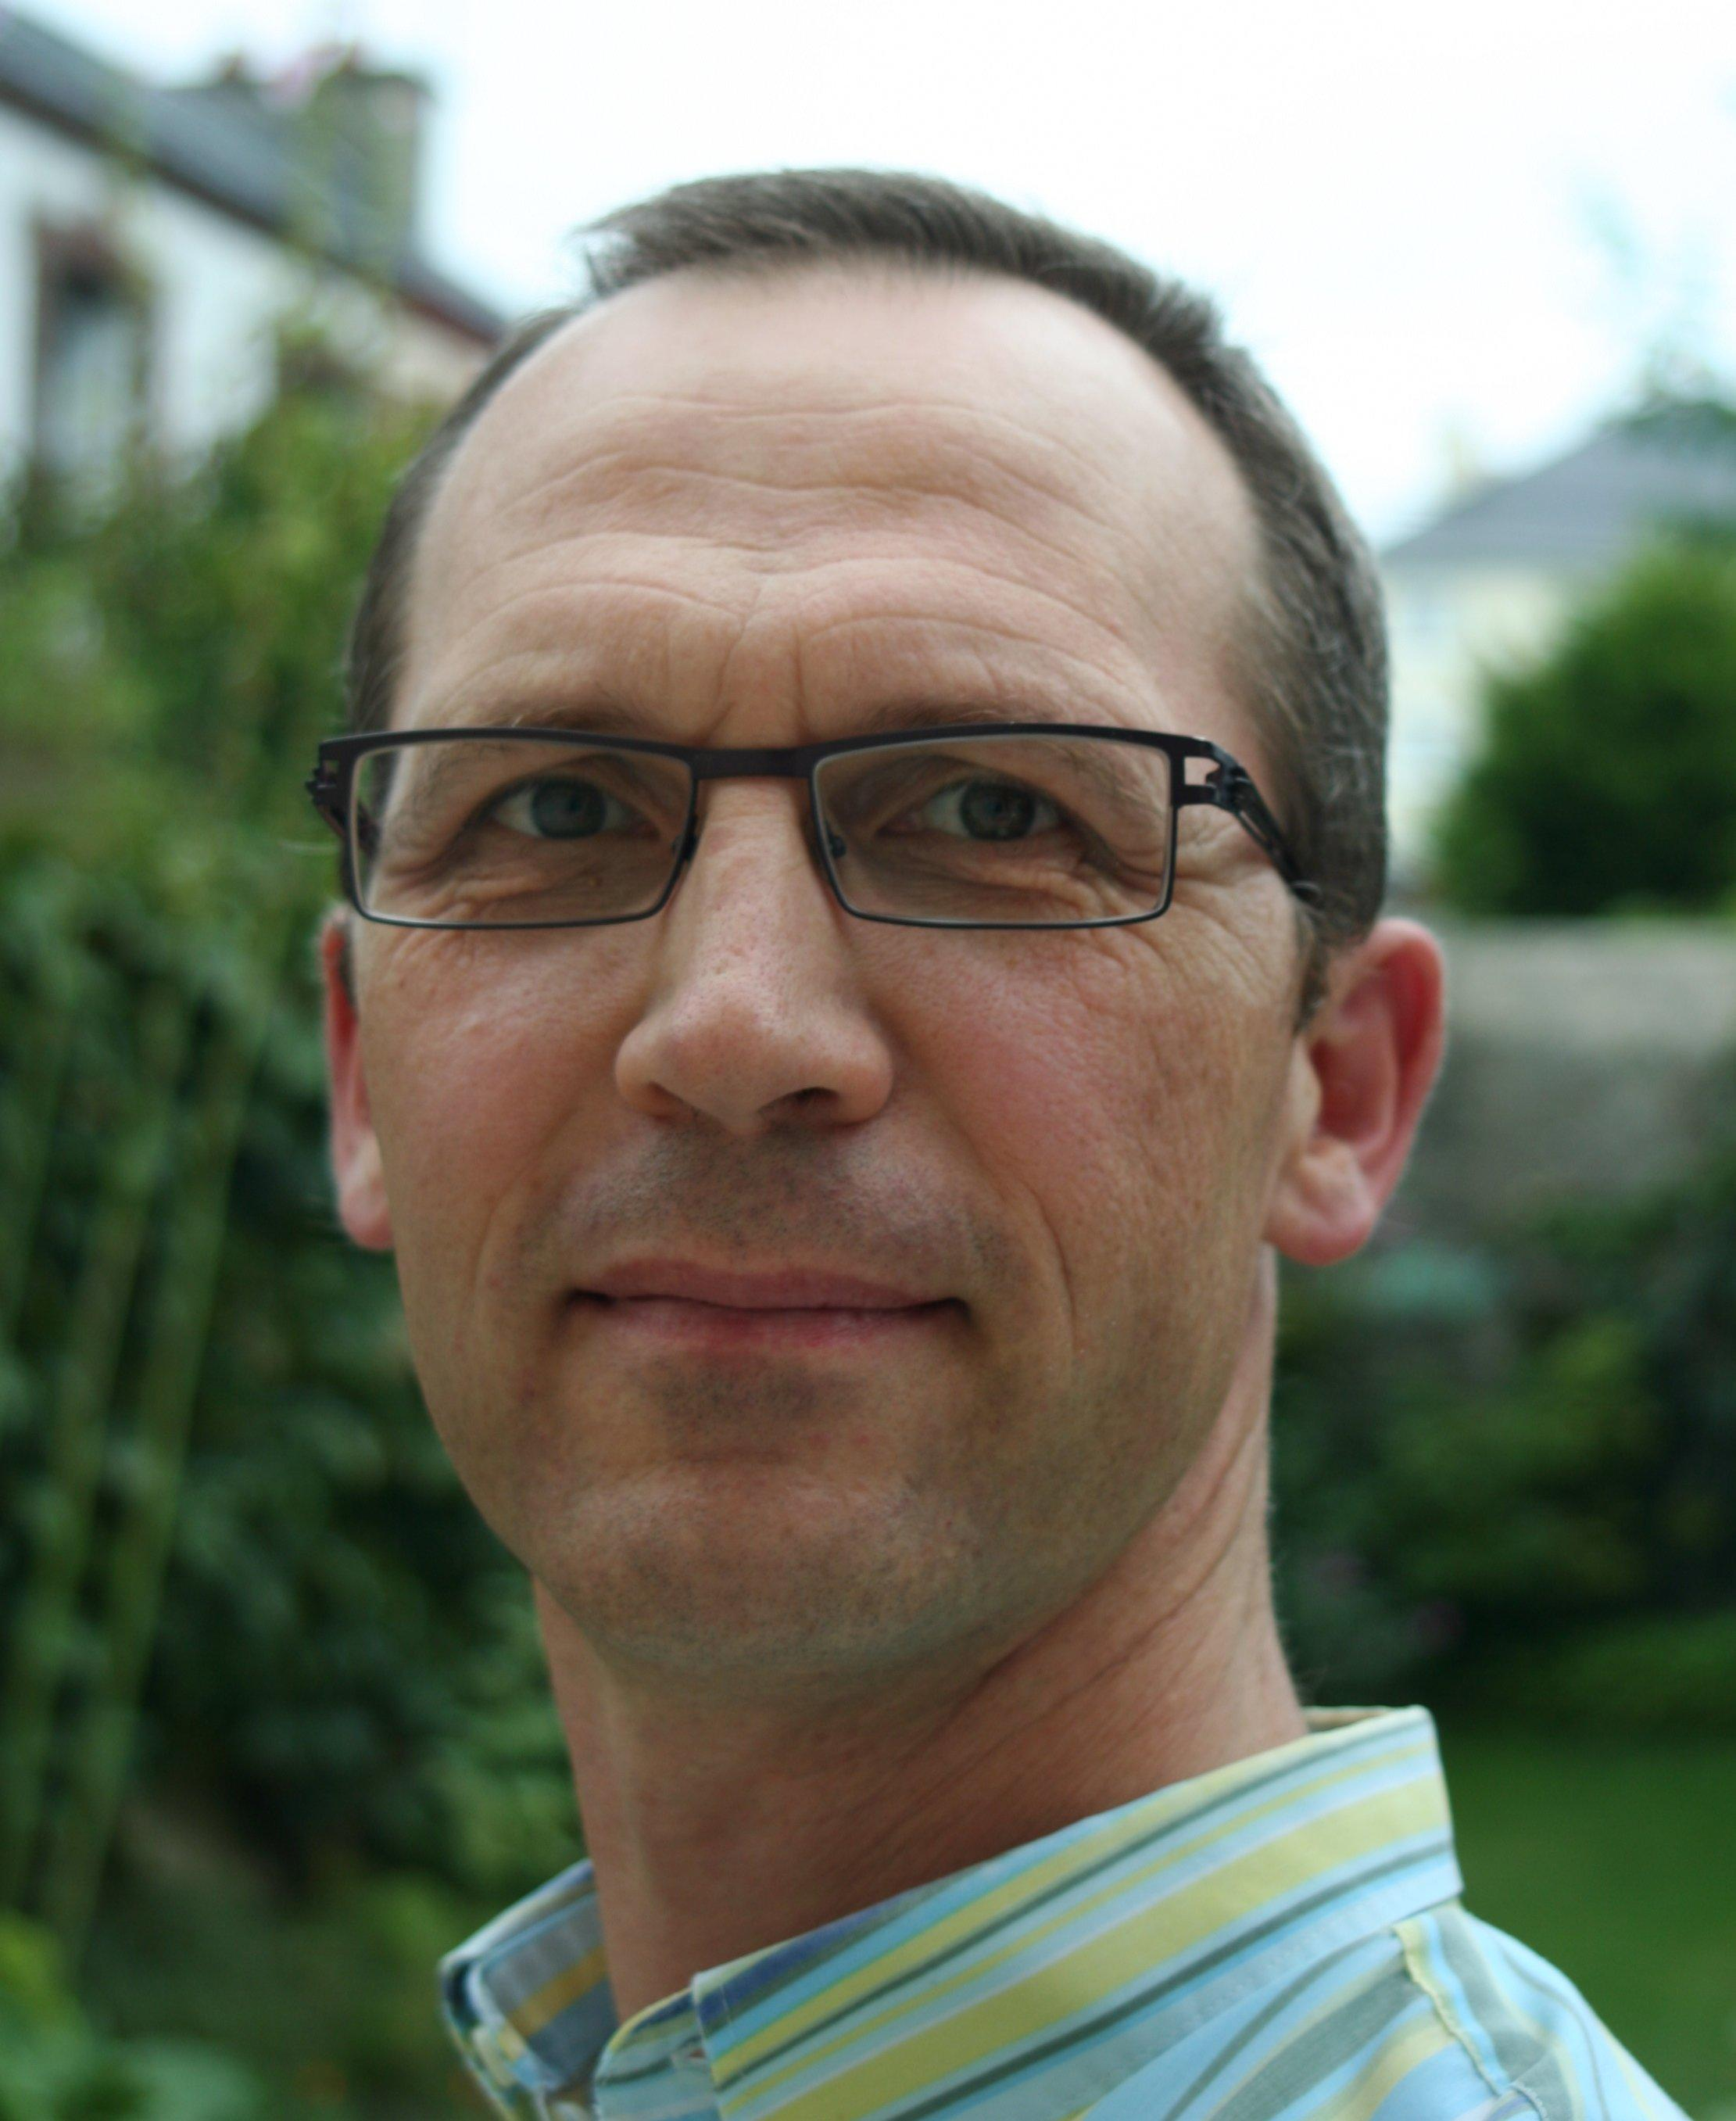
\includegraphics[width=.2\columnwidth]{Pictures/VL.jpeg}}
\end{wrapfigure} 

 \lgf{Vincent Lerouvillois, Assistant pédagogique} 
 \lge{Vincent Lerouvillois, Teaching Assistant}
 

 